\subsection{DSE Parameters}

For our design space exploration, we tested three parameters, word size,
bank size, and maximum fan-in. The word size is the width of the key
memory, which determines how many bits of the key we check at a time in the
key comparison. We tested word sizes of 8, 16, and 32 bits. The bank size is
the size of a bank of the value memory. We test bank sizes of 128 bytes and
256 bytes. The maximum fan-in is the number of bank values that banked
memories multiplex among at every cycle. This, combined with the bank size,
determines the pipeline latency of banked memories. We test max fan-ins of
8 and 16.

In addition to the hardware parameters, we also different target clock periods
to see their effect on power and area. We test a minimum clock period of 0.75 ns,
which roughly corresponds to 10Gb ethernet, a clock period of 1.6 ns,
a clock period of 8 ns, which corresponds to 1Gb ethernet, and a clock period
of 80 ns, which corresponds to 100Mb ethernet. 

\subsection{Results}

\begin{figure}
    \begin{center}
        \includegraphics[width=\linewidth]{dse_slow/powerVSarea.png}
        \caption{1GbE Power vs. Area}
        \label{fig:slow-pva}
    \end{center}
\end{figure}

\begin{figure}
    \begin{center}
        \includegraphics[width=\linewidth]{dse_fast/powerVSarea.png}
        \caption{10GbE Power vs. Area}
        \label{fig:fast-pva}
    \end{center}
\end{figure}

As seen in the figures \ref{fig:slow-pva} and \ref{fig:fast-pva}, our
parameters don't have much affect on power and area. For instance, in Figure
\ref{fig:slow-pva}, the power draw changes by less than a mW, while total
power consumption is around 30 mW. Similarly, area only changes by 600 \(um^2\),
while the total area around 400,000 \(um^2\).

\begin{figure}
    \begin{center}
        \includegraphics[width=\linewidth]{dse_all/powerVSarea.png}
        \caption{All Clocks Power vs. Area}
        \label{fig:all-pva}
    \end{center}
\end{figure}

The real difference comes from changing clock speed. As seen in Figure
\ref{fig:all-pva}, decreasing the clock period from 0.75 ns to 8 ns leads to
a large decrease in both power and area. As shown in Figure 
\ref{fig:all-pva}, the 5Gbps, 1Gbps, and 100Mbps designs create a roughly-pareto
optimal curve. However, we lose this optimiality when attempting to push the
design to a 0.75ns clock for 10Gbps ethernet. 


